\documentclass[handout,11pt]{beamer}

% Choose how your presentation looks.
%
% For more themes, color themes and font themes, see:
% http://deic.uab.es/~iblanes/beamer_gallery/index_by_theme.html
%
\mode<presentation>
{%
	\usetheme{Darmstadt}      % or try Darmstadt, Madrid, Warsaw, ...
	\usecolortheme{beaver} % or try albatross, beaver, crane, ...
	\usefonttheme{serif}  % or try serif, structurebold, ...
	\setbeamertemplate{navigation symbols}{}
	\setbeamertemplate{caption}[numbered]
}

% *** Formatting Packaages ***
\usepackage{bookmark}

% *** Citation Packages ***
\usepackage[citecounter,labelnumber,backend=biber,bibencoding=utf8,sorting=none]{biblatex}
\addbibresource{./bibliography.bib}

% *** Code Blocks Packages ***
\usepackage{listings}
\usepackage{xcolor}
%New colors defined below
\definecolor{codegreen}{rgb}{0,0.6,0}
\definecolor{codegray}{rgb}{0.5,0.5,0.5}
\definecolor{codepurple}{rgb}{0.58,0,0.82}
\definecolor{backcolour}{rgb}{1.0,1.0,1.0}
\lstset{%
	frame=tb,
	backgroundcolor=\color{backcolour},
	commentstyle=\color{codegreen},
	keywordstyle=\color{magenta},
	numberstyle=\tiny\color{codegray},
	stringstyle=\color{codepurple},
	basicstyle=\ttfamily\tiny,
	breakatwhitespace=false,
	breaklines=true,
	captionpos=b,
	keepspaces=true,
	numbersep=5pt,
	numbers=left,
	showspaces=false,
	showstringspaces=false,
	showtabs=false,
	tabsize=2,
}
% *** Diagram Drawing ***
\usepackage{tikz}
\usetikzlibrary{arrows.meta}
% *** File Organization Packages ***
\usepackage{subfiles}
% *** FONT PACKAGES ***
\usepackage[T1]{fontenc}
% *** MATH PACKAGES ***
\usepackage{amsmath}
\interdisplaylinepenalty=2500
\usepackage{amssymb}
% *** GRAPHICS PACKAGES ***
\usepackage[export]{adjustbox} % Frame around figures (via the frame option in includegraphic)
\usepackage{array}
\usepackage{graphicx}
\usepackage{media9}
\usepackage[font=small,skip=0pt]{caption}
\usepackage{tabularx}
\usepackage{subcaption}
\setlength{\marginparwidth}{2cm}
\usepackage{todonotes}

% *** Table Packages ***
\usepackage{multirow}

% *** Unsorted Packages ***
\usepackage[absolute,overlay]{textpos}
	\setlength{\TPHorizModule}{1mm}
	\setlength{\TPVertModule}{1mm}
%\newcolumntype{b}{X}
\newcolumntype{s}{>{\hsize=.5\hsize}X}


% Title Page Info %%%%%%%%%%%%%%%%%%%%%%%%%%%%%%
\title{Context-Aware Malware Detection Using Topic Modeling}
\author[W. Stegner]{A Thesis Presented By: Wayne Stegner}
\date{\today}
\institute[]{%
	\normalsize
	Committee Members: \\
	Dr.\ Rashmi Jha (Chair) \\
	Dr.\ Carla Purdy \\
	Dr.\ David Kapp \\
	Dr.\ Temesguen Kebede
}
\logo{
\includegraphics[height=1.0cm]{img/uc_logo.png}}

% Start of Document
\begin{document}
	% New Section %%%%%%%%%%%%%%%%%%%%%%%%%%%%%%
	\section{Introduction}
	\begin{frame}
		\centering
		\titlepage{}
	\end{frame}
	\begin{frame}{Acknowledgements}
		This work was funded by AFRL under DAGSI-SOCHE Award No. RY8-UC-20-1.
	\end{frame}
	\begin{frame}{Motivation}
		\begin{itemize}
			\item Need for cyber security is growing
			\item SolarWinds cyber attack
				\begin{itemize}
					\item Malware attack compromised an estimated 100 companies and
						several U.S.\ federal agencies
					\item Could cost hundreds of millions of dollars to U.S.\ government
						alone
				\end{itemize}
			\item Colonial Pipeline cyber attack
				\begin{itemize}
					\item Major U.S.\ oil pipeline was compromised
					\item Pipeline operation temporarily halted
				\end{itemize}
			\item Severe consequences: Need better understanding of cyber threats
		\end{itemize}
	\end{frame}
	\begin{frame}{Motivation for Context}
		\begin{itemize}
			\item A given action is not malicious by nature
			\item Malice is relative to the desired outcome
			\item Sort vs.\ search programs
				\begin{itemize}
					\item Searching: Changing the data is unexpected
					\item Sorting: Reordering is expected (but not changing actual
						values)
				\end{itemize}
			\item Autonomous drone camera shutoff
				\begin{itemize}
					\item Turning off a drone's camera is not always malicious
					\item But it \textit{can} be malicious
					\item Depends on the context
				\end{itemize}
		\end{itemize}
	\end{frame}

	\section{Background}
	\begin{frame}{Malware Analysis Overview}
		\begin{itemize}
			\item Static analysis
				\begin{itemize}
					\item Examining the file without running it
					\item Opcodes, system calls, control flow features, etc.
					\item Difficult if code is obfuscated
				\end{itemize}
			\item Dynamic analysis
				\begin{itemize}
					\item Examining the file by running it
					\item Opcodes, system calls, control flow, system changes, network
						activity, etc.
					\item Requires sandbox environment to contain malware
				\end{itemize}
		\end{itemize}
	\end{frame}
	\begin{frame}{k-Nearest Neighbors (k-NN)}
		\begin{itemize}
			\item Simple machine learning classification algorithm
			\item Only parameter --- $k$, the number of neighbors
			\item Present labeled training dataset
			\item Inference the class of new points
				\begin{itemize}
					\item Majority vote among the $k$ nearest neighbors to the new point
					\item Typically uses Euclidean distance
				\end{itemize}
		\end{itemize}
	\end{frame}
	\begin{frame}{Latent Dirichlet Allocation (LDA)}
		\begin{itemize}
			\item Generative statistical topic modeling
				algorithm~\cite{bleiLatentDirichlet2003}
			\item Learn latent topics from a corpus of documents
				\begin{itemize}
					\item Each topic is a probability distribution over the vocabulary
				\end{itemize}
			\item Assign weighted mixture of topics to each document
			\item Bag-of-words (BoW) preprocessing
				\begin{itemize}
					\item Document: ``cat dog mouse cat cat dog''
					\item BoW\@: $\{``cat'': 3, ``dog'': 2, ``mouse'': 1\}$
				\end{itemize}
		\end{itemize}
	\end{frame}
	\begin{frame}{LDA Model Evaluation}
		\begin{itemize}
			\item Intrinsic evaluation
				\begin{itemize}
					\item Directly measure quality of topics
					\item Perplexity or topic cohesion
					\item Unsupervised methods (do not need labeled data)
				\end{itemize}
			\item Extrinsic evaluation
				\begin{itemize}
					\item Evaluate topic quality through secondary task
					\item Classification accuracy
					\item Can be more intuitive to interpret
				\end{itemize}
		\end{itemize}
	\end{frame}
	\begin{frame}{LDA in Malware Classification}
		\begin{itemize}
			\item API calls~\cite{sundarkumarMalwareDetection2015}
				\begin{itemize}
					\item Modeled topics from API calls with LDA
					\item Classified topic distributions using various classifiers
					\item Maximum accuracy of 98.61\%
				\end{itemize}
			\item Static/dynamic opcodes~\cite{greerUnsupervisedInterpretable2019}
				\begin{itemize}
					\item Modeled topics from both static and dynamic opcode sequences
						using LDA
					\item Showed difference between search and sort programs using LDA
						topic distributions
					\item Analysis was done manually
				\end{itemize}
			\item Static opcodes~\cite{djaneye-boundjouStaticAnalysis2019a}
				\begin{itemize}
					\item Extends~\cite{greerUnsupervisedInterpretable2019} to include
						malware classification
					\item Classified Microsoft Malware Classification Challenge (BIG
						2015)~\cite{ronenMicrosoftMalware2018} using k-NN
					\item Accuracy of 97.2\%
				\end{itemize}
		\end{itemize}
	\end{frame}
	\begin{frame}{Context in Software Analysis}
		\begin{itemize}
			\item Context-based access control~\cite{%
					fernandezContextsContextbased2007,
					shebaroContextbasedAccess2015,
				}
				\begin{itemize}
					\item Limit allowed actions based on location data
					\item Targets smartphone security
				\end{itemize}
			\item Interaction-based context~\cite{shresthaTapwaverubLightweight2015}
				\begin{itemize}
					\item Require user gestures to allow sensitive actions
					\item Targets smartphone security
				\end{itemize}
			\item Graph-based context~\cite{narayananContextawareAdaptive2017}
				\begin{itemize}
					\item Examine entry point of program representation graphs
					\item Include whether the user is aware or unaware of the action
					\item Targets smartphone security
				\end{itemize}
		\end{itemize}
	\end{frame}

	\section{Methodology}
	\begin{frame}{Threat Model}
		\centering
		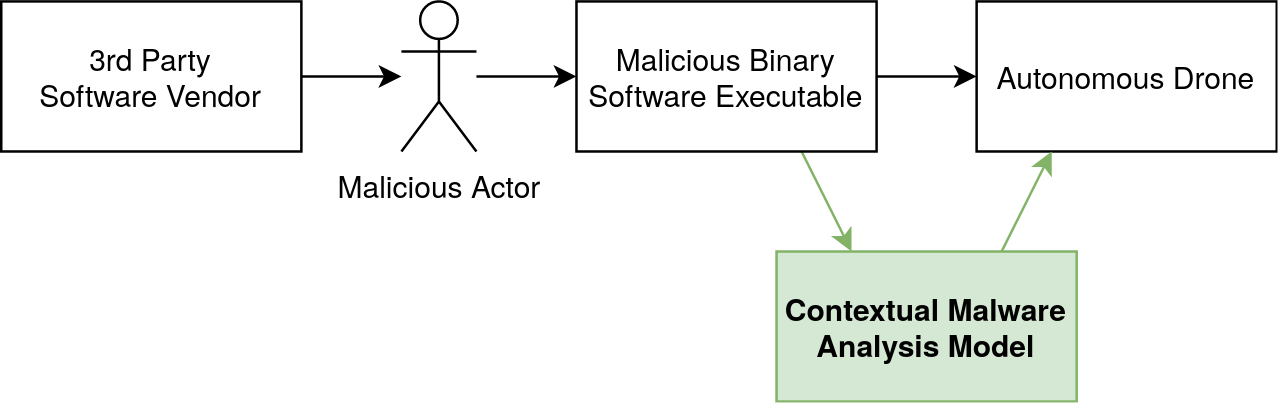
\includegraphics[width=0.85\textwidth]{img/threat_model.png}
	\end{frame}
	\begin{frame}{Context Definition}
		\begin{itemize}
			\item Context should encapsulate:
				\begin{enumerate}
					\item What is the physical context of the system?
					\item How does actual behavior compare to expected behavior?
					\item Why is the software making certain decisions?
				\end{enumerate}
		\end{itemize}
	\end{frame}
	\begin{frame}{Cross Validation}
		\begin{itemize}
			\item LDA models have high randomness
				\begin{itemize}
					\item Accuracy variations of several percent on the same data
					\item Difficult to compare parameters
				\end{itemize}
			\item Solve with k-fold cross validation
				\begin{itemize}
					\item Split dataset into $k$ folds
					\item Cycle through folds as testing partitions
					\item $k$ different models trained
					\item Take average performance
				\end{itemize}
		\end{itemize}
	\end{frame}

	\subsection{Context-Free Model}
	\begin{frame}{Model Overview}
		\begin{itemize}
			\item Purpose of the model
				\begin{itemize}
					\item Extrinsic evaluation of LDA features
					\item Explore model parameters (number of topics and $k$)
				\end{itemize}
			\item Input data
				\begin{itemize}
					\item Each file is a sequence of static opcodes
				\end{itemize}
			\item Evaluated using 5-fold cross validation
		\end{itemize}
	\end{frame}
	\begin{frame}{Model Process}
		\begin{enumerate}
			\item Transform all documents into BoW documents.
			\item Fit LDA model on the training partition.
			\item Transform all BoW documents into topic distributions.
			\item Fit k-NN classifier on the topic distributions of the training
				partition.
			\item Evaluate k-NN classifier on the topic distributions of the test
				partition.
		\end{enumerate}
	\end{frame}

	\subsection{Context Bit Model}
	\begin{frame}{Model Overview}
		\begin{itemize}
			\item Utilize static, dynamic, and behavioral features
			\item Extract useful features with LDA/BoW models
			\item Define context based on physical context
				\begin{itemize}
					\item Environment data collected from sensors
					\item Simplified to a single bit (good vs bad context)
				\end{itemize}
		\end{itemize}
	\end{frame}
	\begin{frame}{Ensemble Model Diagram}
		\centering
		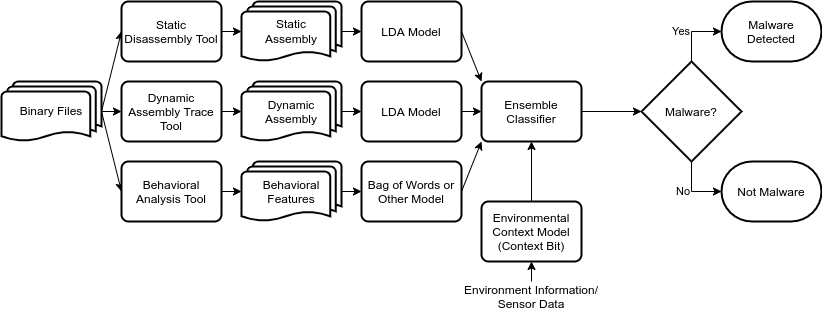
\includegraphics[width=0.95\textwidth]{img/system_diagram_ensemble_context_bit.png}
	\end{frame}
	\begin{frame}{Simplifications}
		\begin{itemize}
			\item There is a lot going on
				\begin{itemize}
					\item Three different feature extraction methods required
				\end{itemize}
			\item Dynamic features are difficult to collect
				\begin{itemize}
					\item Difficult to make malware run in a sandbox
					\item Took a \textit{long} time to collect
				\end{itemize}
			\item Simplified model to use only static features
		\end{itemize}
	\end{frame}
	\begin{frame}{Simplified Model Diagram}
		\centering
		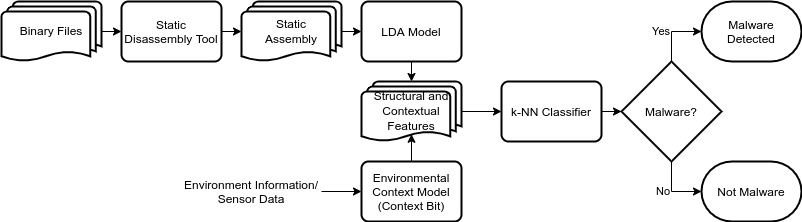
\includegraphics[width=0.95\textwidth]{img/system_diagram_simple_context_bit.png}
	\end{frame}
	\begin{frame}{Context Integration}
		\begin{itemize}
			\item Randomly generate context bit for each file
			\item Append context bit to LDA topic vector
				\begin{itemize}
					\item With 15 topics, feature vector is 16-dimensional
				\end{itemize}
			\item Label whether or not the physical context matches the action (file
				class)
				\begin{itemize}
					\item Benign file with good context is operating within proper
						context
					\item Malicious file with bad context is operating within proper
						context
					\item Other cases, file is violating its context
				\end{itemize}
		\end{itemize}
	\end{frame}
	\begin{frame}{Dataset --- Das Malwerk}
		\begin{itemize}
			\item Dataset requirements
				\begin{itemize}
					\item Small dataset for initial testing
					\item Live files for dynamic analysis
						\begin{itemize}
							\item This requirement was later dropped
						\end{itemize}
				\end{itemize}
			\item Two class dataset
				\begin{itemize}
					\item Malicious files --- 576 samples from Das
						Malwerk~\cite{svenssonMalwerk}
					\item Benign files --- 646 samples from default Windows 7
						installation
				\end{itemize}
		\end{itemize}
	\end{frame}

	\subsection{Expected Behavior Model}
	\begin{frame}{Model Overview}
		\begin{itemize}
			\item Similar to simplified context bit model
				\begin{itemize}
					\item Utilize static disassembly features with LDA
					\item Only difference is context definition
				\end{itemize}
			\item Define context based on expected behavior
				\begin{itemize}
					\item What type of software do we expect?
					\item In practice --- vendor description of the software
					\item For testing --- class label in the dataset
				\end{itemize}
		\end{itemize}
	\end{frame}
	\begin{frame}{Dataset --- BIG 2015}
		\begin{itemize}
			\item Limitations of Das Malwerk dataset
				\begin{itemize}
					\item Only two classes: malicious and benign
					\item Classes are too general
				\end{itemize}
			\item New dataset --- BIG 2015~\cite{ronenMicrosoftMalware2018}
				\begin{itemize}
					\item Nine classes separated by specific functionality
					\item Already disassembled
				\end{itemize}
			\item We are not treating these files as inherently malicious
				\begin{itemize}
					\item Yes, these are all technically malware
					\item Treated as just nine different types of software
				\end{itemize}
		\end{itemize}
	\end{frame}
	\begin{frame}{Context Integration}
		\begin{itemize}
			\item Goal --- simulate receiving software that is not the type we expect
			\item Change 50\% of the class labels
				\begin{itemize}
					\item Class label represents expected software type
				\end{itemize}
			\item Append new class label to LDA feature vector
				\begin{itemize}
					\item One-hot encoding ---
						$3 \rightarrow \{0, 0, 1, 0, 0, 0, 0, 0, 0\}$
					\item With 15 LDA topics, feature vector is 24-dimensional
				\end{itemize}
			\item Label whether or not context is violated
				\begin{itemize}
					\item File with changed label is violating its context
					\item File with original label is operating within proper context
				\end{itemize}
		\end{itemize}
	\end{frame}

	\section{Results}
	\subsection{Context-Free Model}
	\begin{frame}{Classification Accuracy --- Das Malwerk}
		\centering
		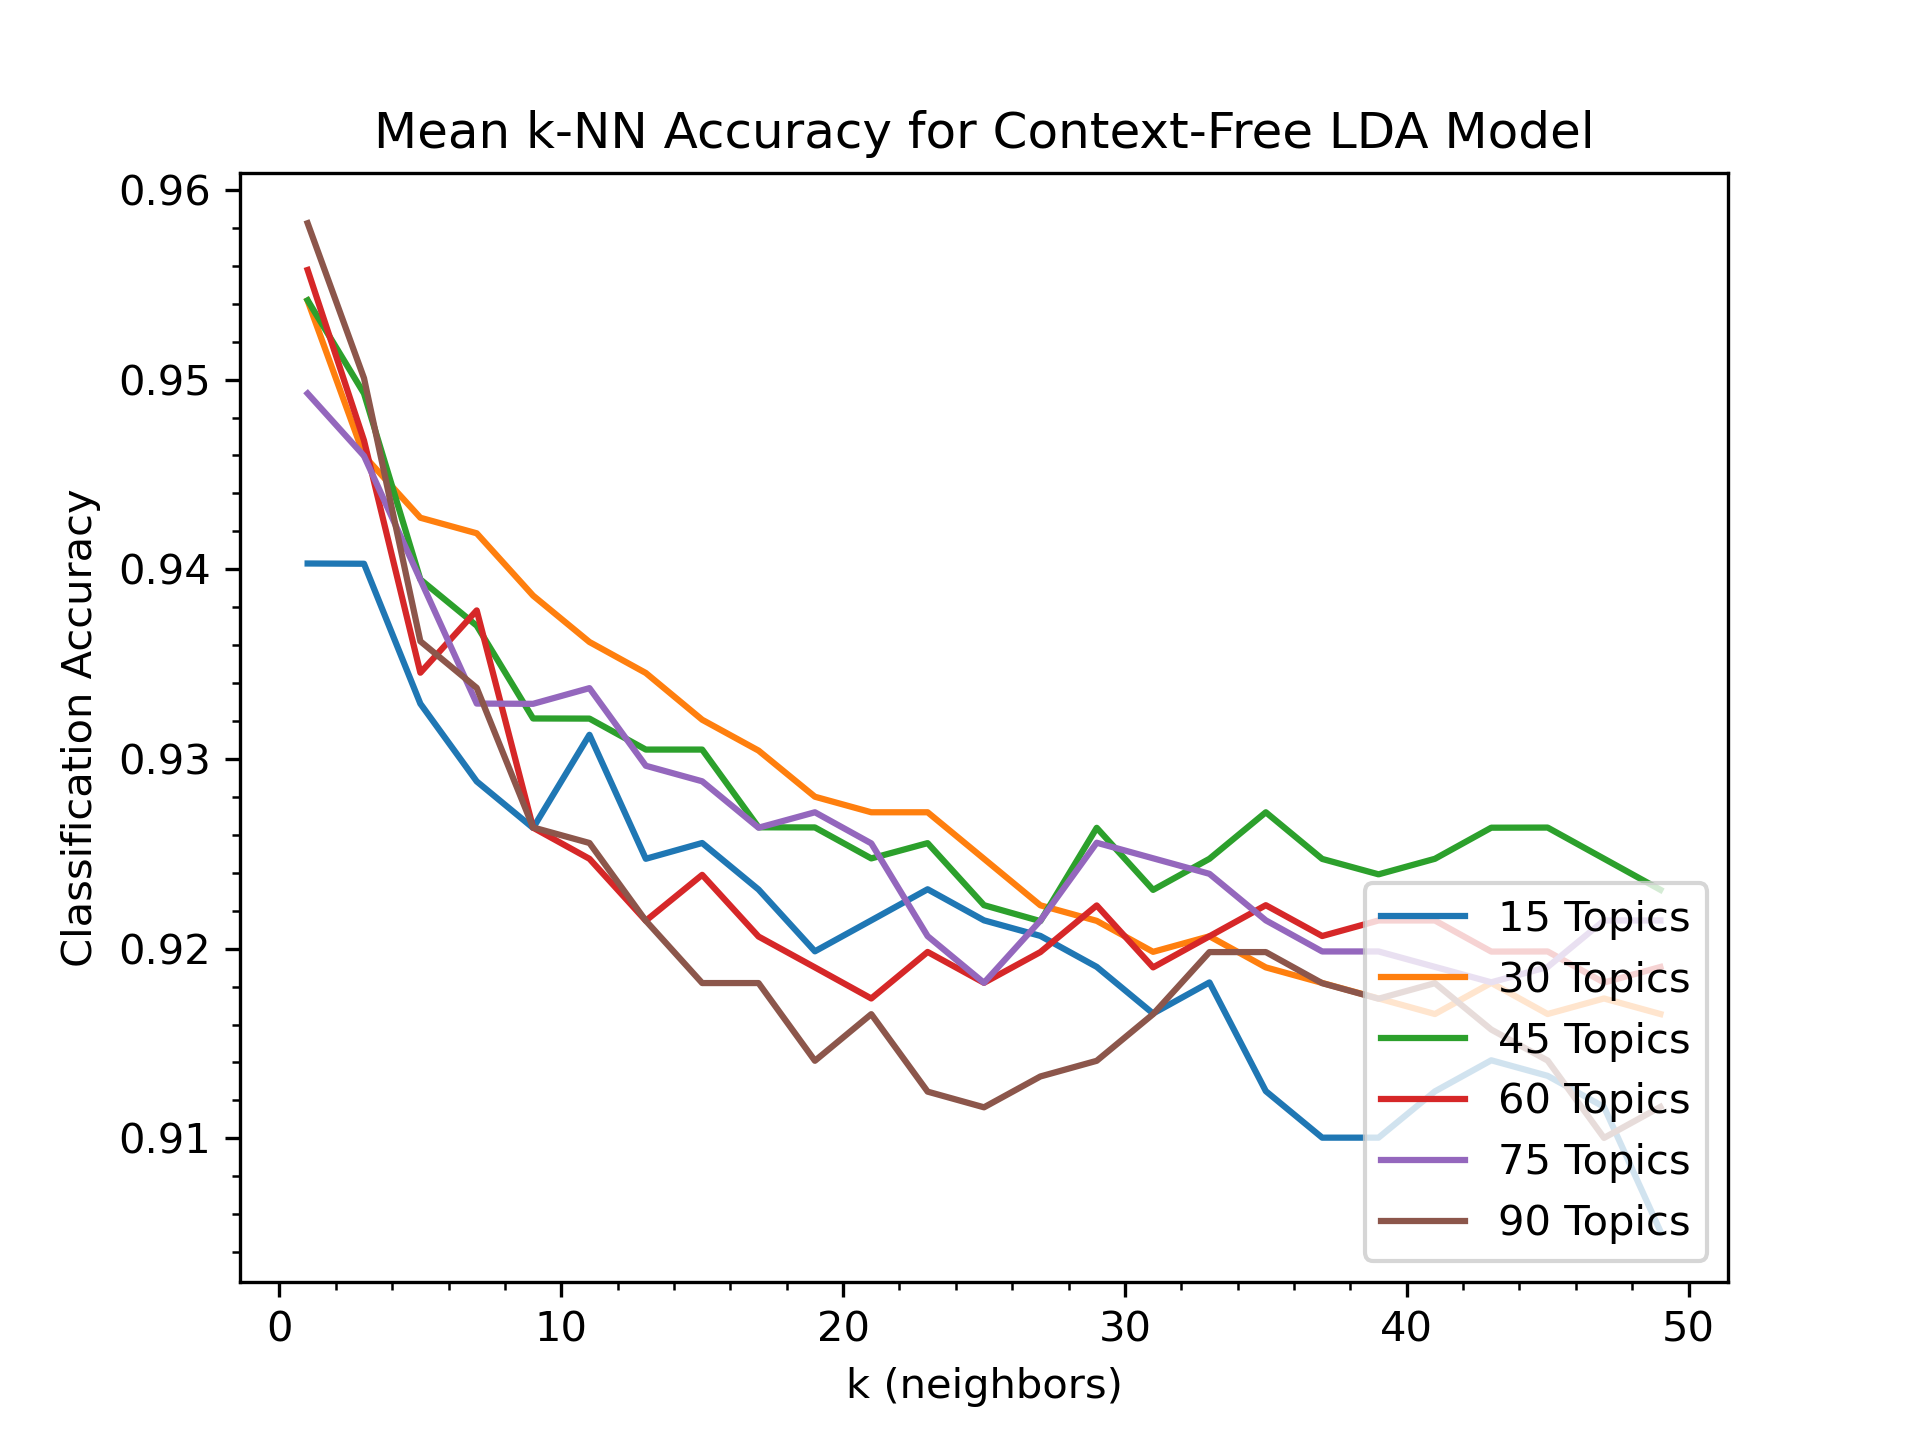
\includegraphics[width=0.85\textwidth]{img/win32/knn_lda.png}
	\end{frame}
	\begin{frame}{Classification Accuracy --- Das Malwerk}
		\centering
		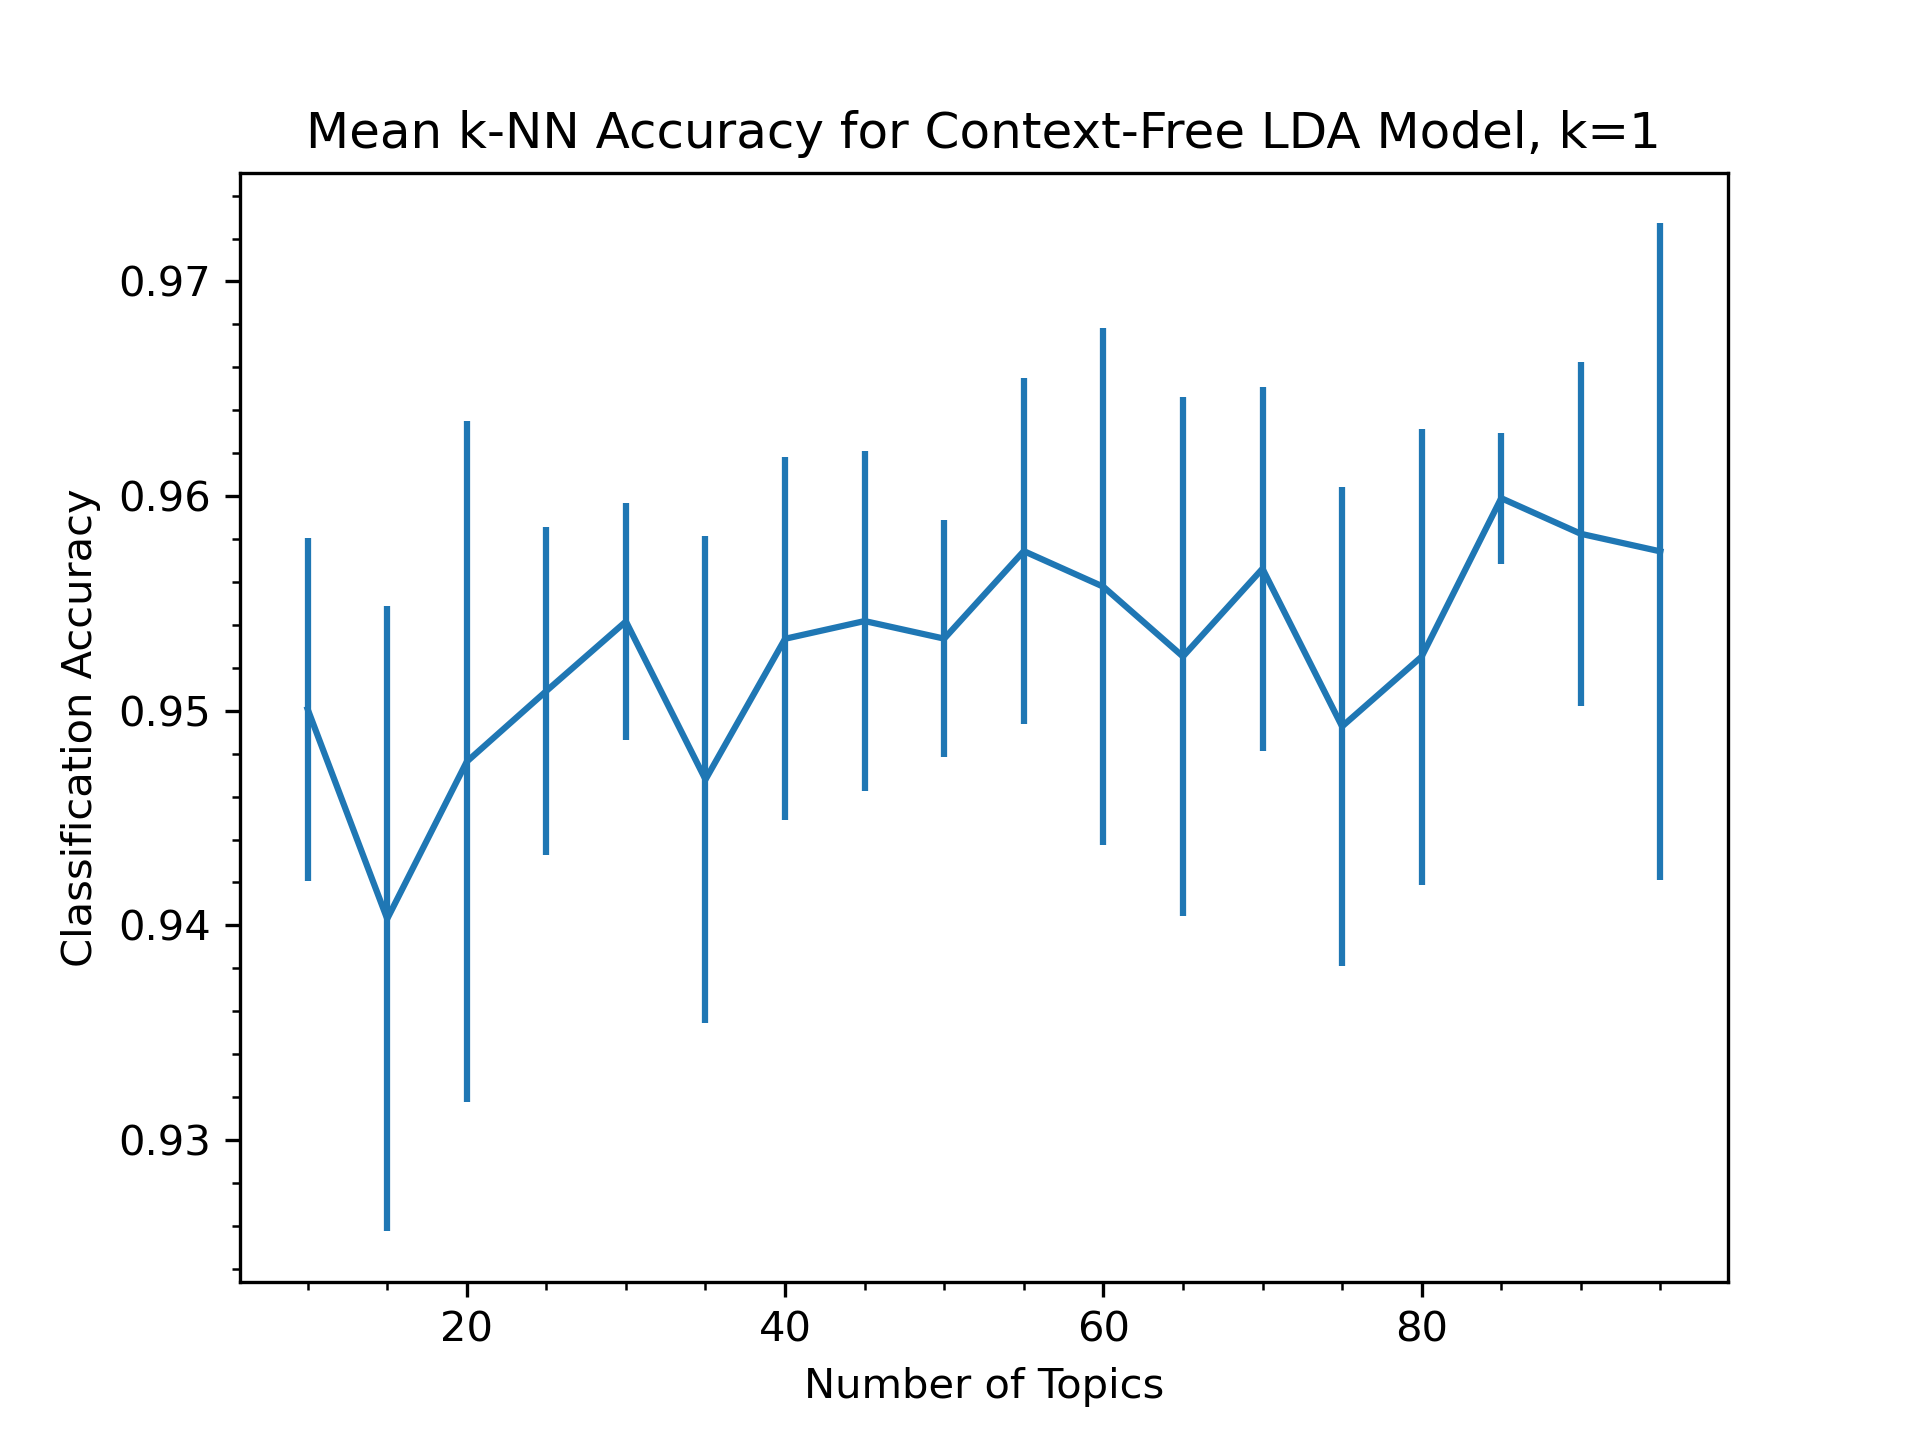
\includegraphics[width=0.85\textwidth]{img/win32/knn_lda_k_01.png} \\
		Best accuracy: 85 LDA topics, $k=1$ --- 95.99\%
	\end{frame}
	\begin{frame}{Classification Accuracy --- BIG 2015}
		\centering
		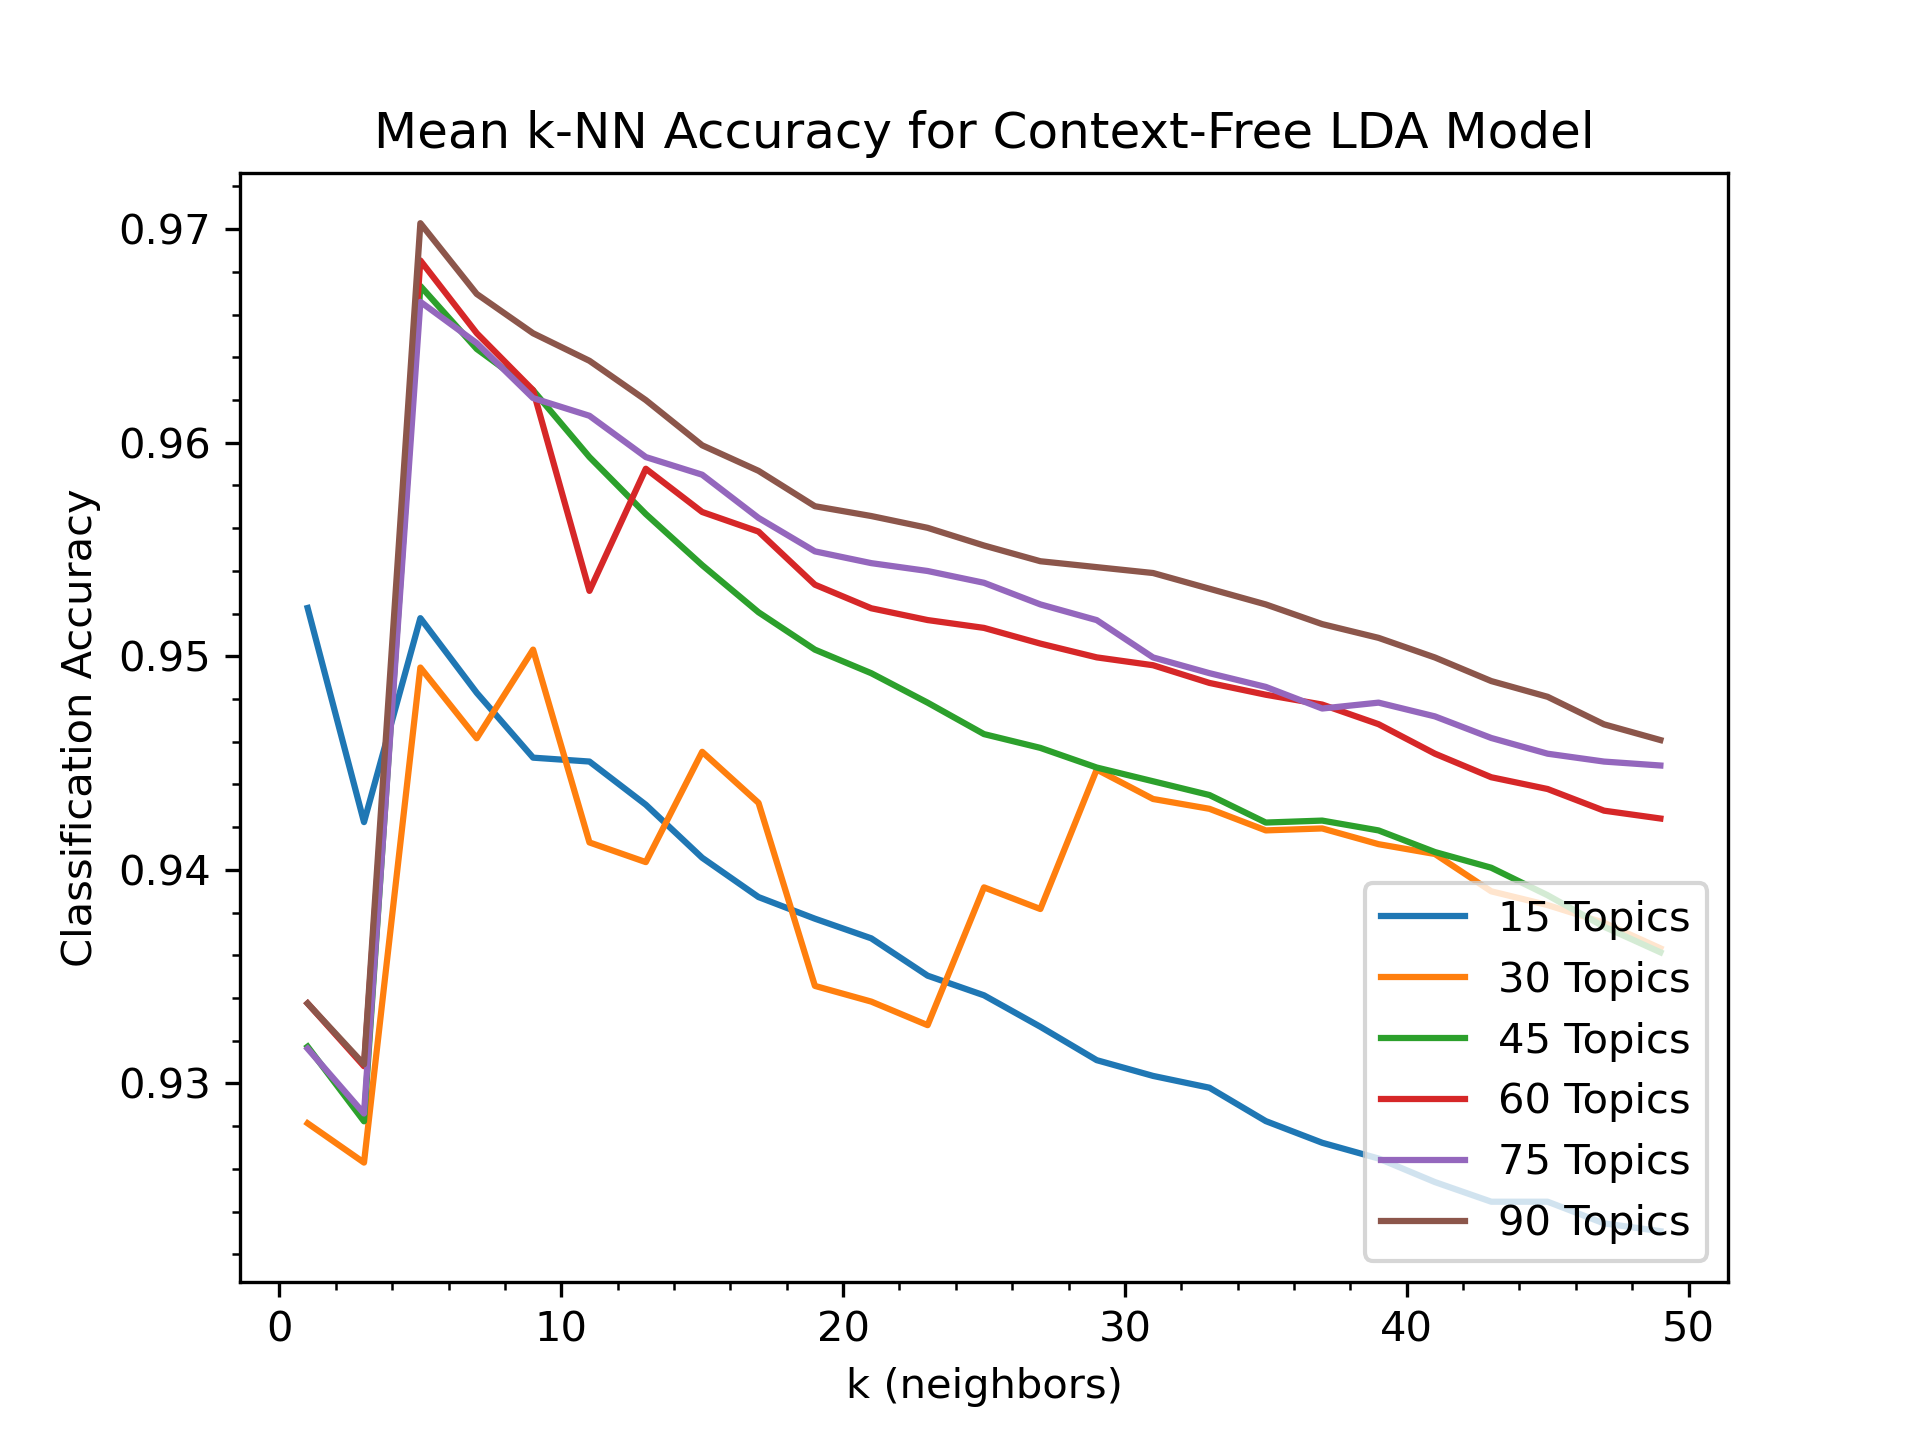
\includegraphics[width=0.85\textwidth]{img/msoft_big/knn_lda.png}
	\end{frame}
	\begin{frame}{Classification Accuracy --- BIG 2015}
		\centering
		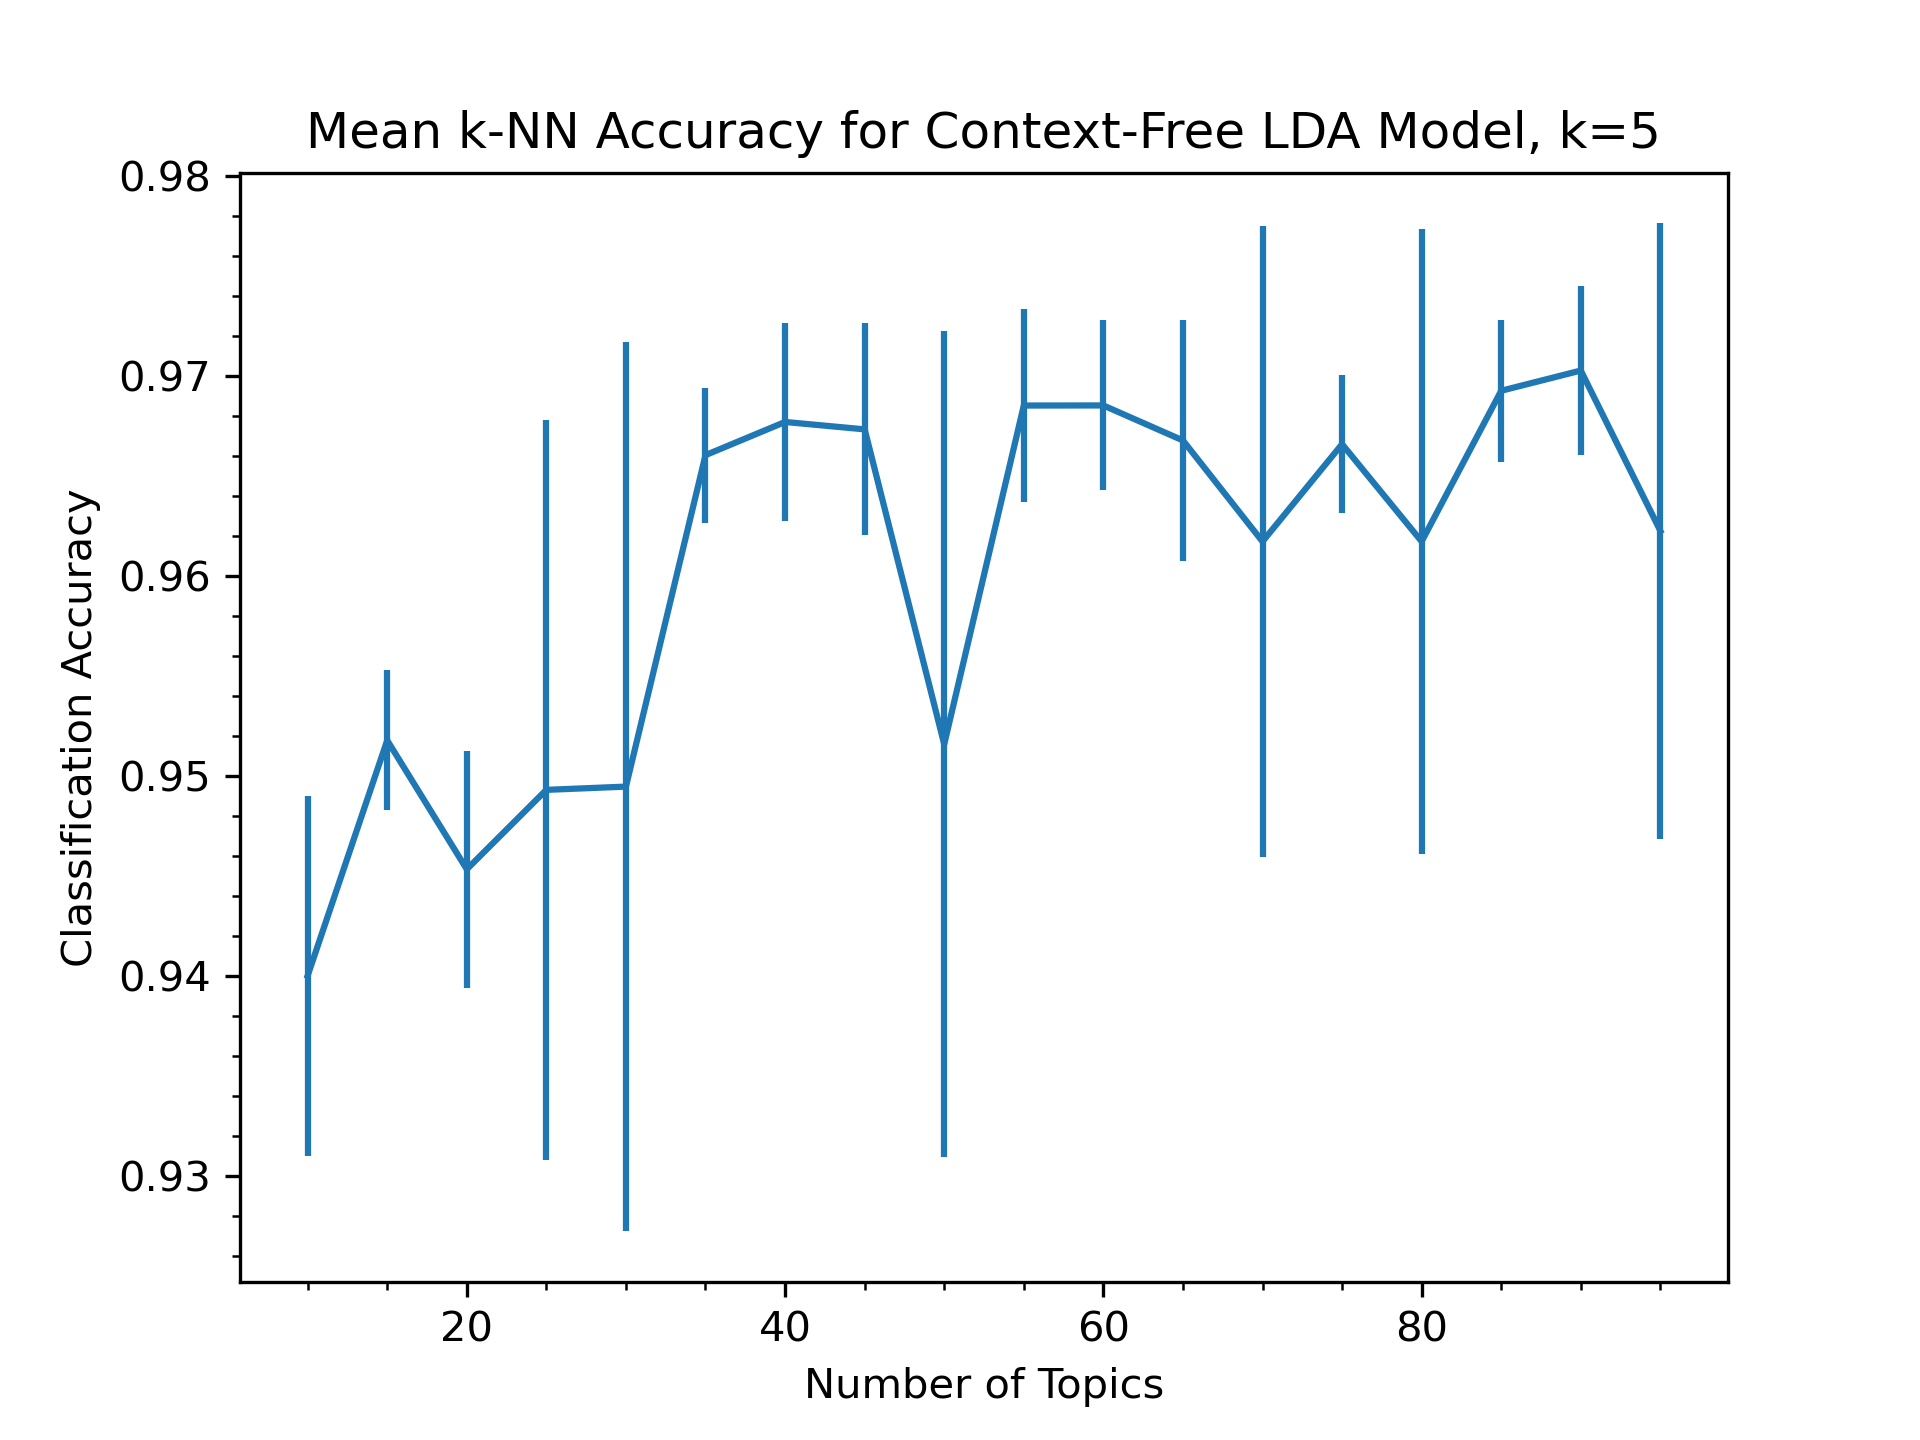
\includegraphics[width=0.85\textwidth]{img/msoft_big/knn_lda_k_05.png} \\
		Best accuracy: 90 LDA topics, $k=5$ --- 97.03\%
	\end{frame}
	\begin{frame}{Discussion}
		\begin{itemize}
			\item Good performance on both datasets
				\begin{itemize}
					\item LDA features carry useful information for classification
				\end{itemize}
			\item Large error bars
				\begin{itemize}
					\item High variance between models with the same parameters
					\item Cannot be confident our best parameters are actually the best
				\end{itemize}
		\end{itemize}
	\end{frame}

	\subsection{Context Bit Model}
	\begin{frame}{Classification Accuracy}
		\centering
		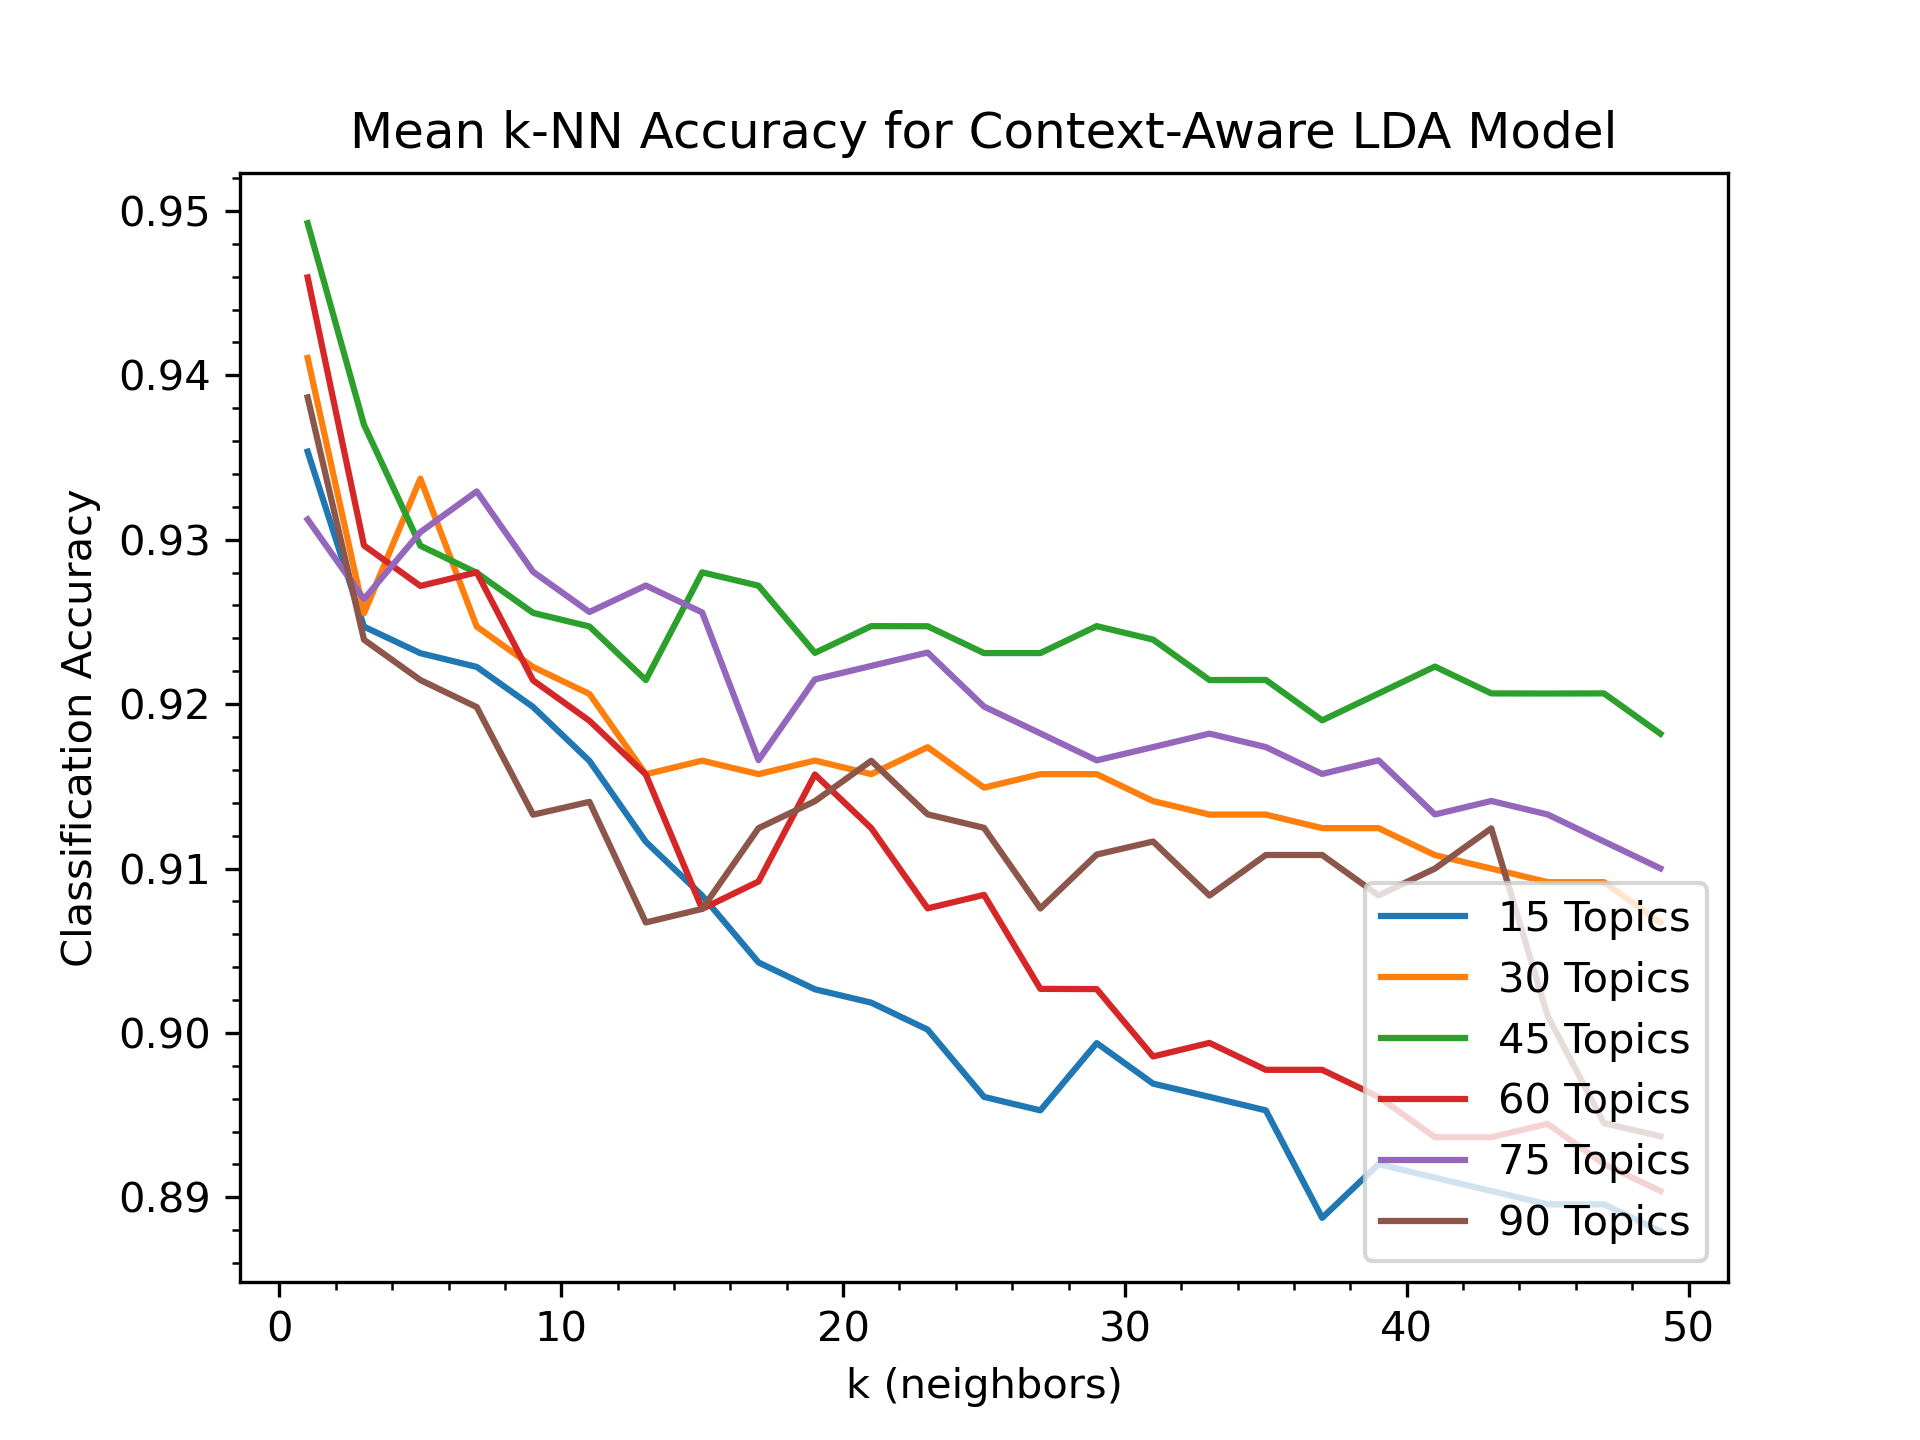
\includegraphics[width=0.85\textwidth]{img/win32/knn_lda_context.png}
	\end{frame}
	\begin{frame}{Classification Accuracy}
		\centering
		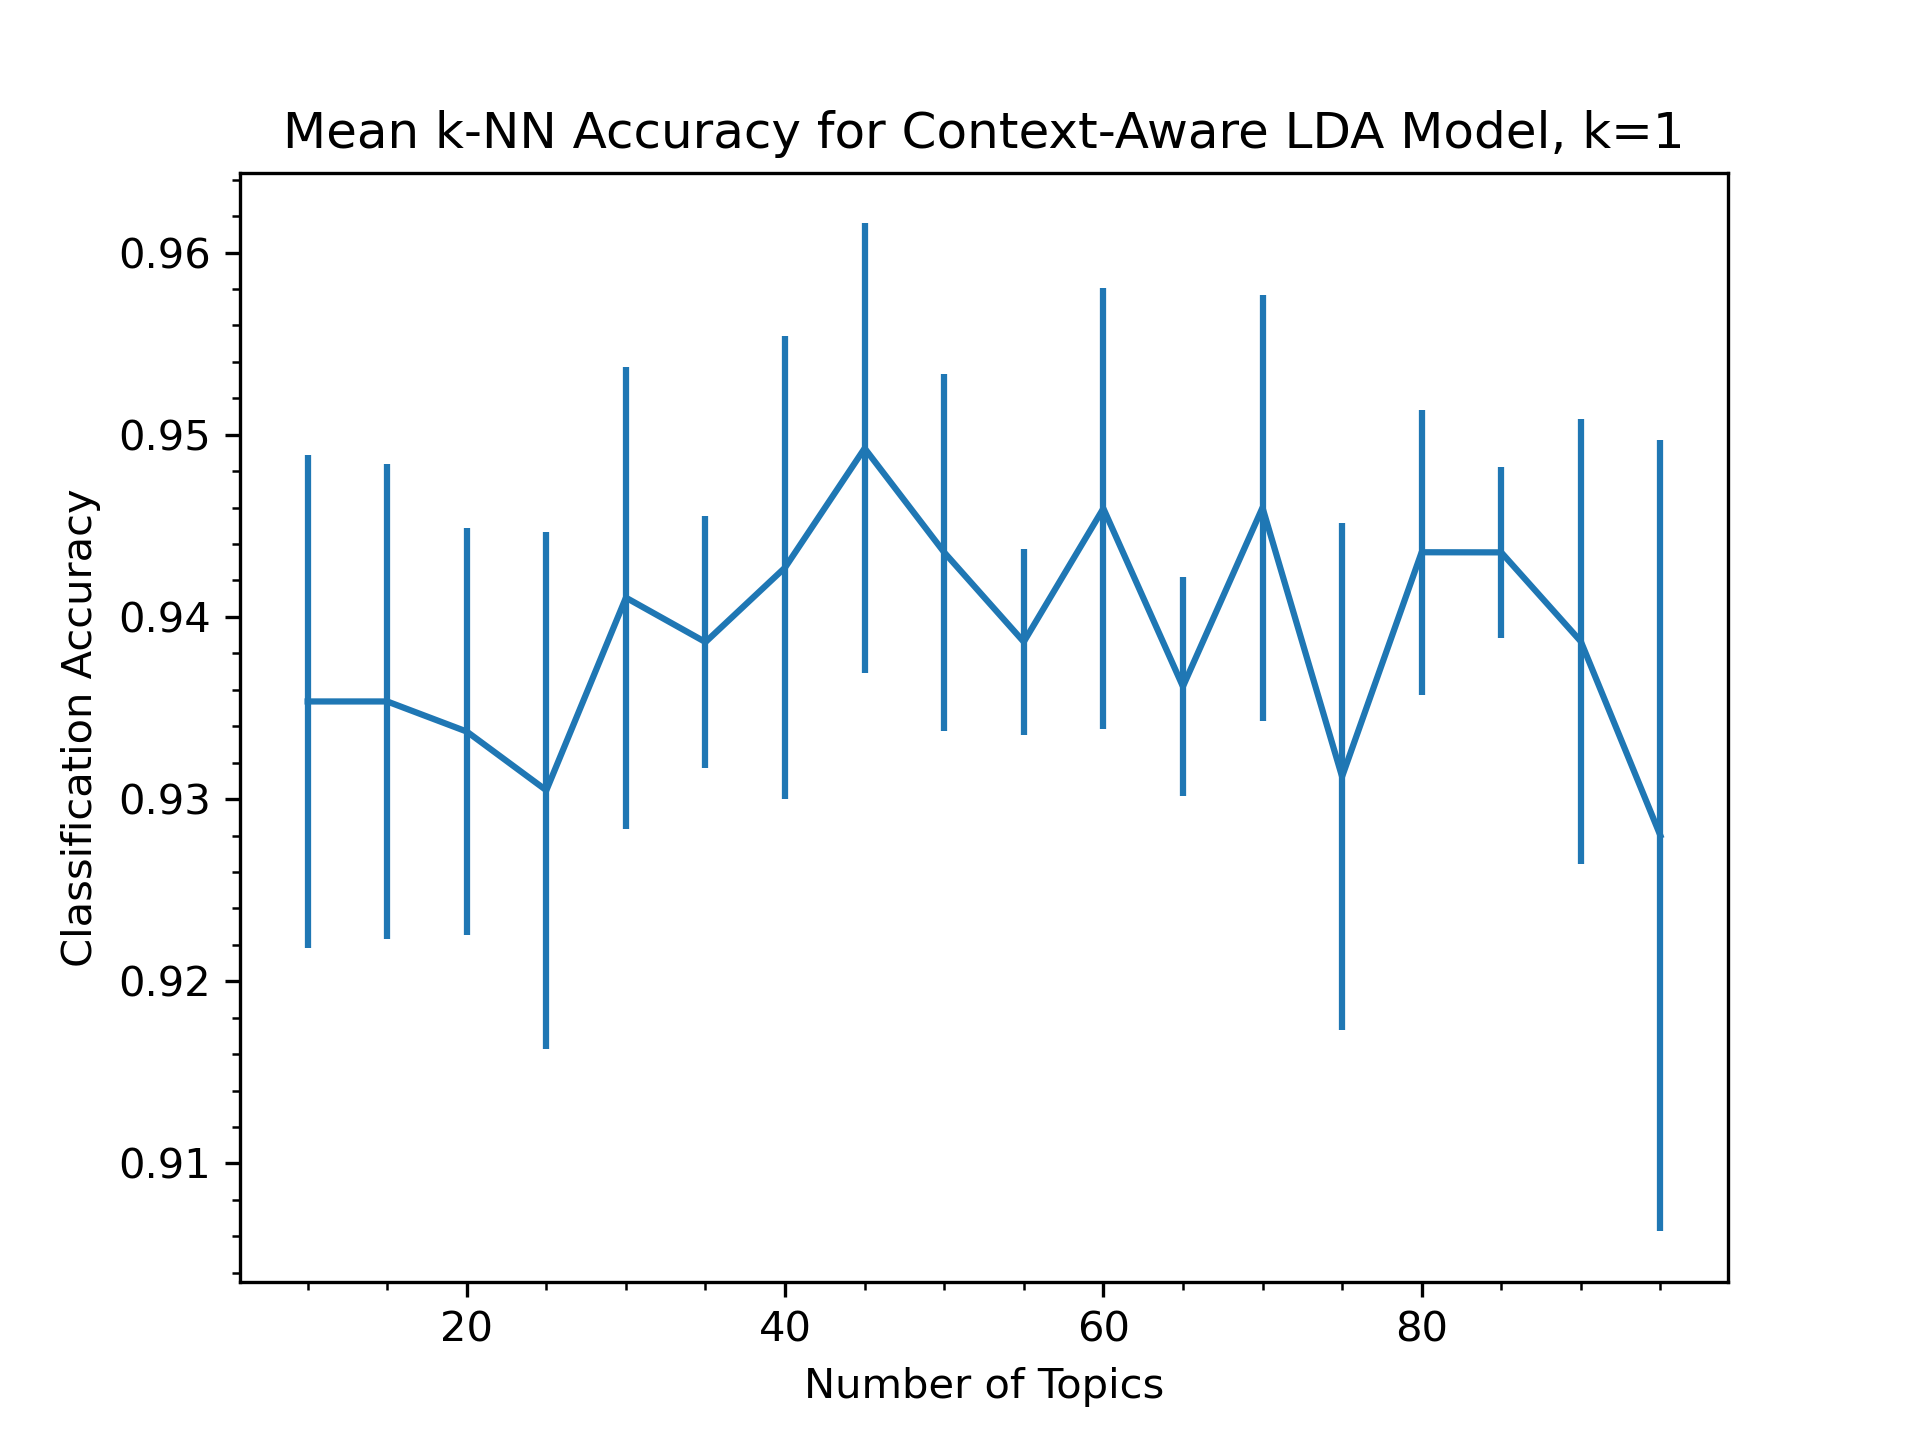
\includegraphics[width=0.85\textwidth]{img/win32/knn_lda_context_k_01.png} \\
		Best accuracy: 45 LDA topics, $k=1$ --- 94.92\%
	\end{frame}
	\begin{frame}{Discussion}
		\begin{itemize}
			\item Good performance for the given task
				\begin{itemize}
					\item Lower than context-free system
					\item Large error bars
				\end{itemize}
			\item Task is oversimplified
				\begin{itemize}
					\item Context is not a single binary value
					\item Require more complex model
				\end{itemize}
			\item Physical context alone does not form complete context
		\end{itemize}
	\end{frame}

	\subsection{Expected Behavior Model}
	\begin{frame}{Classification Accuracy}
		\centering
		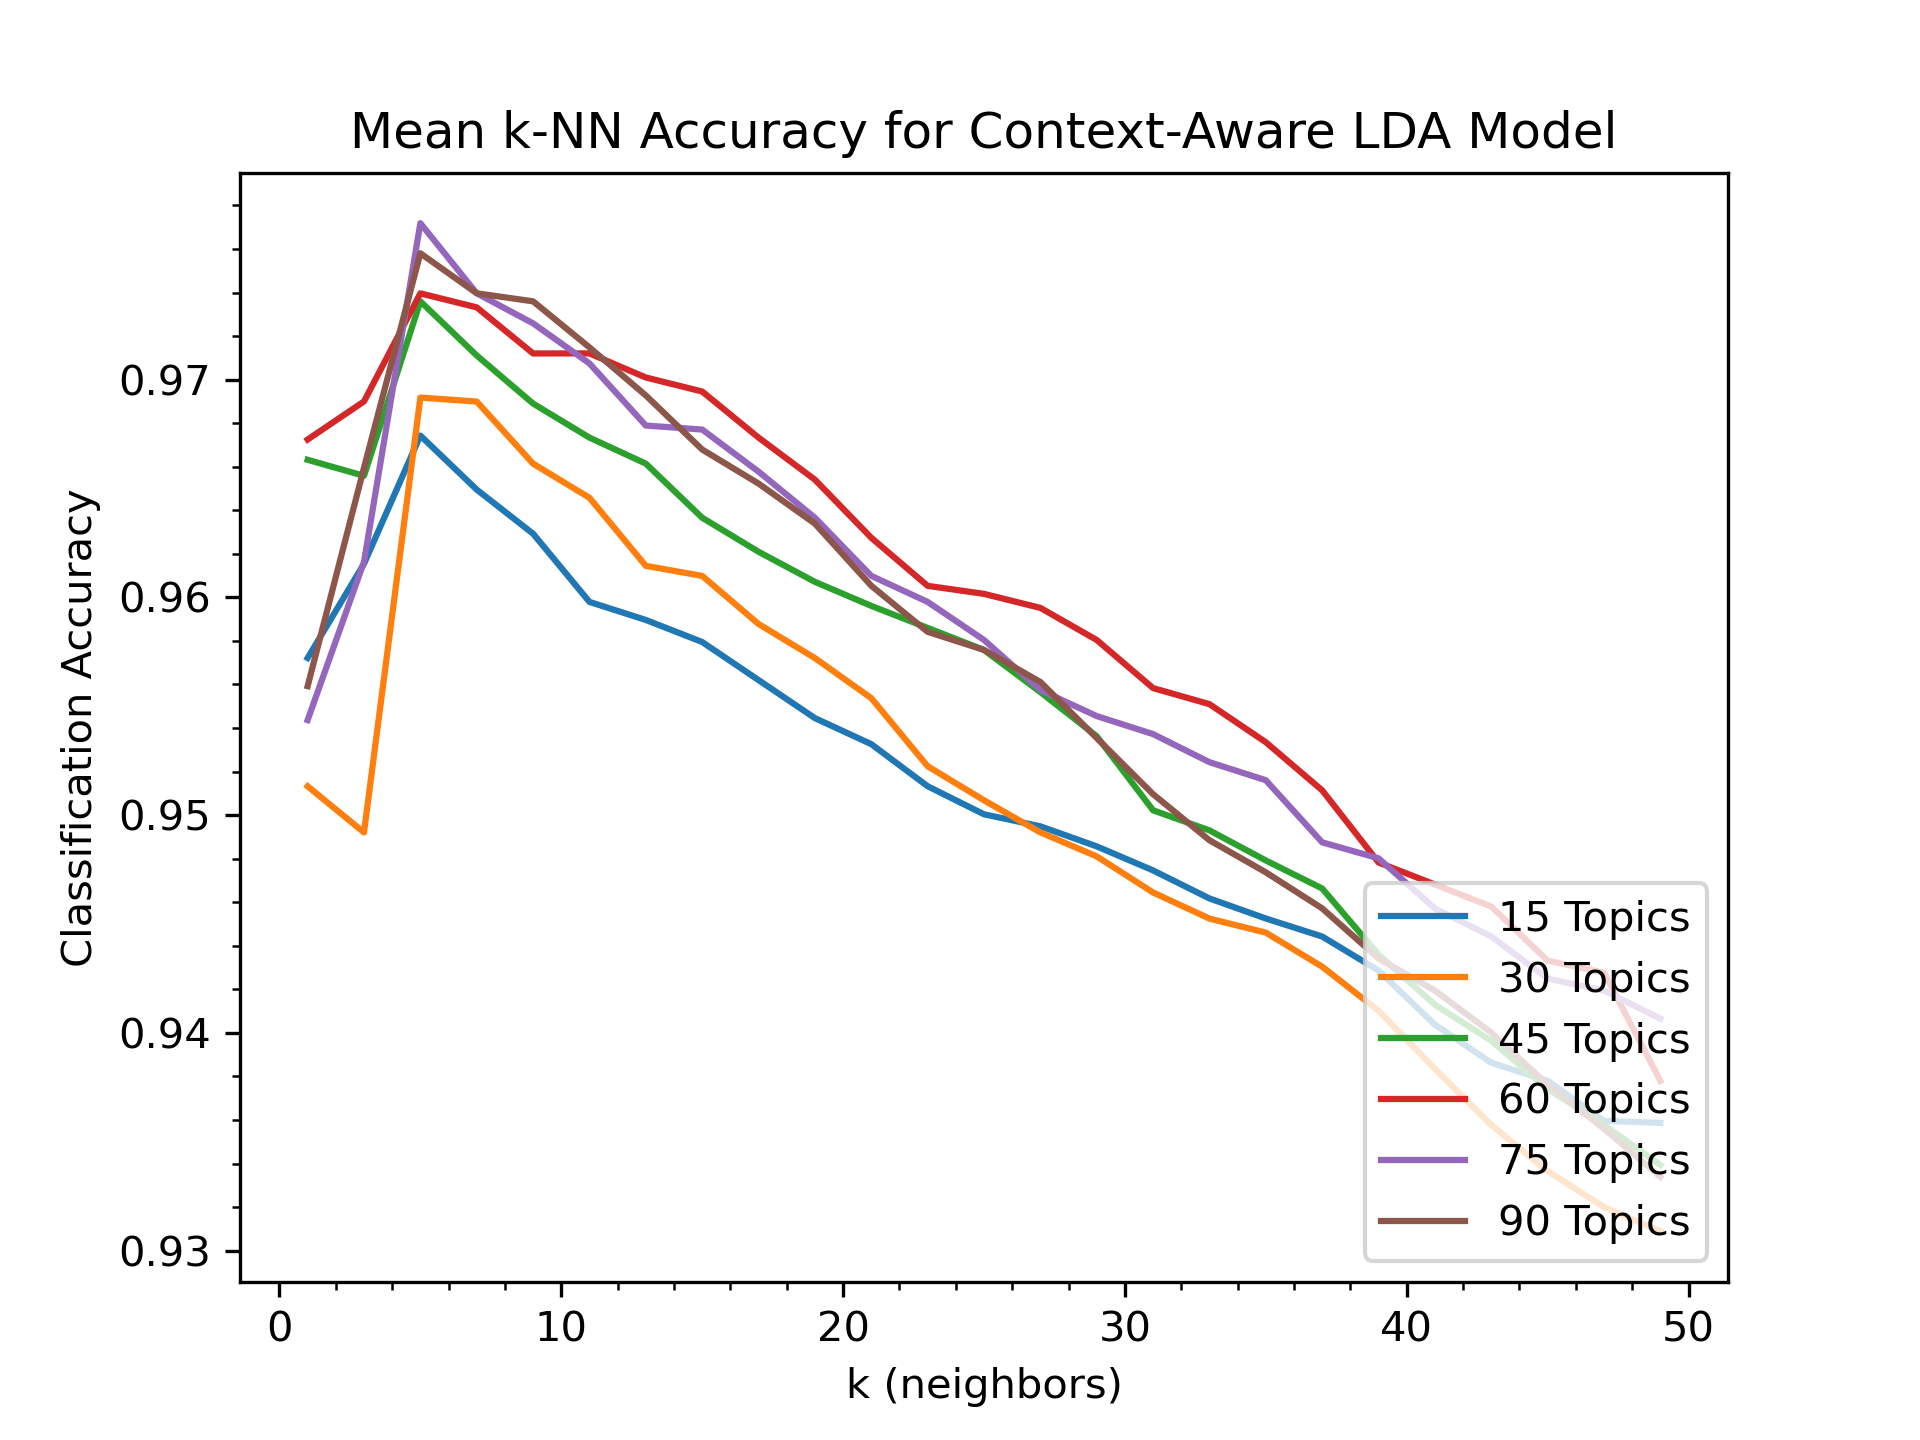
\includegraphics[width=0.85\textwidth]{img/msoft_big/knn_lda_context.png}
	\end{frame}
	\begin{frame}{Classification Accuracy}
		\centering
		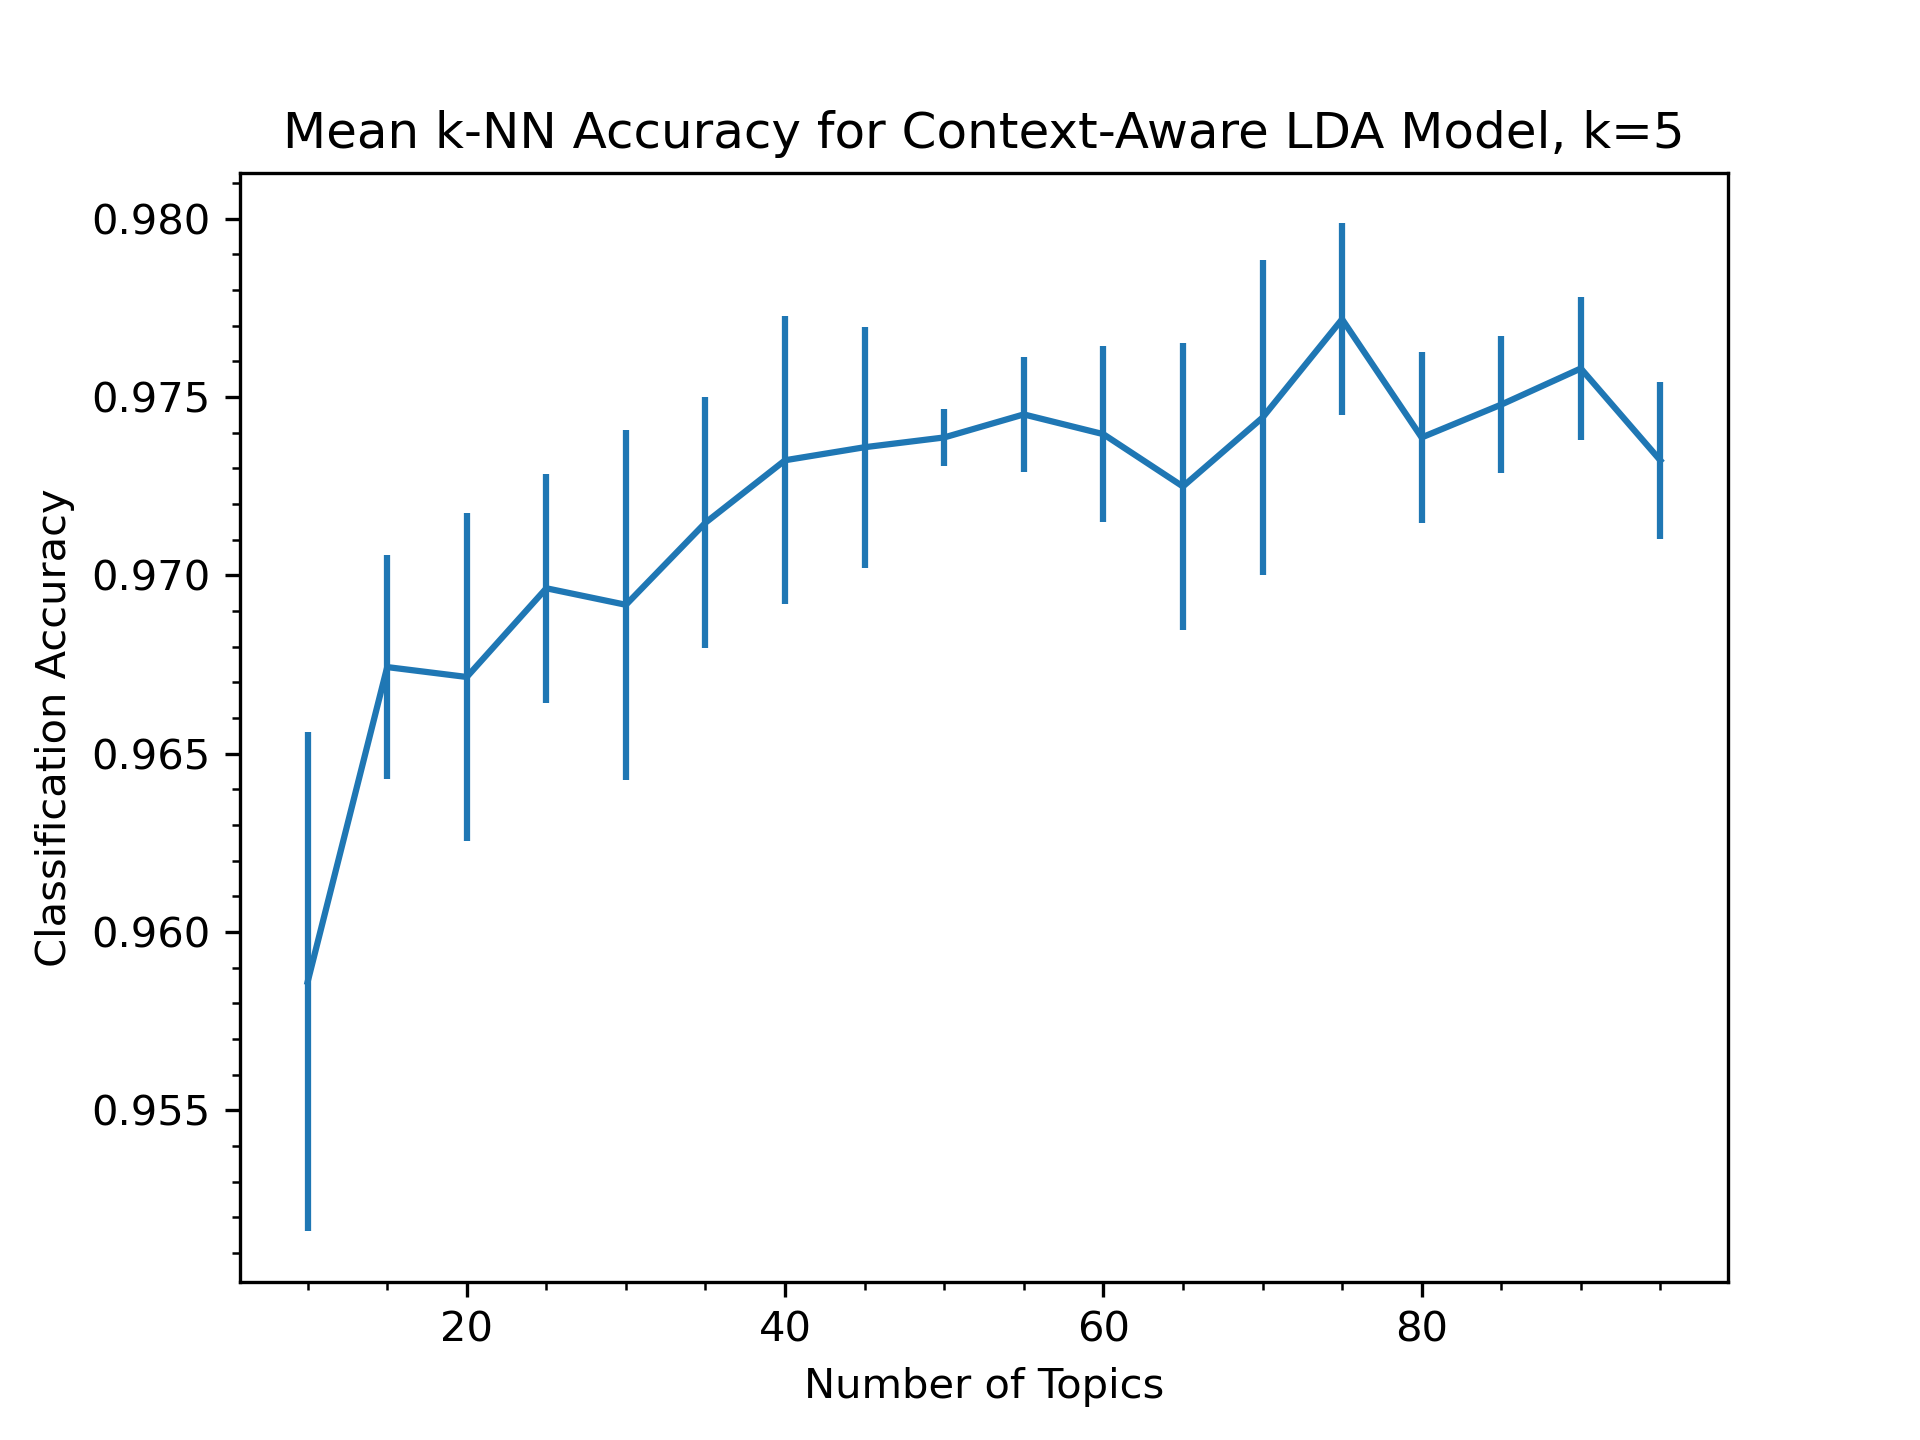
\includegraphics[width=0.85\textwidth]{img/msoft_big/knn_lda_context_k_05.png} \\
		Best accuracy: 75 LDA topics, $k=5$ --- 97.72\%
	\end{frame}
	\begin{frame}{Discussion}
		\begin{itemize}
			\item Good performance on the given task
				\begin{itemize}
					\item Higher than context-free system
					\item Large error bars
				\end{itemize}
			\item Expected behavior may not fit into discrete classes
				\begin{itemize}
					\item Some classes may have similar behaviors
					\item Some programs could be a mixture of classes
				\end{itemize}
		\end{itemize}
	\end{frame}

	\section{Conclusions}
	\begin{frame}{Conclusions}
		\begin{itemize}
			\item Explored the definition of context in malware detection
			\item Presented two proof-of-concept models to address various parts of
				context
			\item Context is challenging to define
				\begin{itemize}
					\item Framing context for software analysis
					\item Our questions do not translate directly to computational model
				\end{itemize}
			\item Proof-of-concept models performed well at their task, but do not
				make a complete picture of context
		\end{itemize}
	\end{frame}
	\begin{frame}{Future Work}
		\begin{itemize}
			\item Add dynamic analysis
			\item Biological inspiration
				\begin{itemize}
					\item Higher-level cognition
				\end{itemize}
			\item Physical context model improvements
			\item Combining context models
			\item More rigorous parameter tuning
		\end{itemize}
	\end{frame}
	\begin{frame}{List of Publications}
		\footnotesize
		\par \hangindent=1cm W\@. Stegner, D\@. Kapp, T\@. Kebede, and R\@. Jha,
		``Context-Aware Malware Detection Using Topic Modeling'', \textit{Submitted
		but not published}.

		\par \hangindent=1cm W\@. Stegner, T\@. Westland, D\@. Kapp, T\@. Kebede,
		and R\@. Jha, ``MiBeX\@: Malware-Inserted Benign Datasets for Explainable
		Machine Learning'', in \textit{Interpretable Artificial Intelligence: A
		Perspective of Granular Computing}, Feb. 2021, pp\@. 269--291.

		\par \hangindent=0.5cm M\@. Santacroce, W\@. Stegner, D\@. Koranek, R\@.
		Jha, ``A Foray Into Extracting Malicious Features from Executable Code with
		Neural Network Salience'', in \textit{2019 IEEE National Aerospace and
		Electronics Conference (NAECON)}, Dayton, OH, USA\@: IEEE, Jul. 2019,
		pp\@. 185--191.

	\end{frame}

	\begin{frame}[allowframebreaks]
		\frametitle{References}
		See thesis for full reference list.
		\printbibliography{}
	\end{frame}
\end{document}
